\subsection{Metric spaces}\label{subsec:metric_spaces}

\begin{definition}\label{def:metric_space}\cite[248]{Engelking1989}
  A \textbf{metric space} is a set \( X \) along with a function \( \mu: X \times X \to \BB{R}^{\geq 0} \), called a \textbf{metric} or \textbf{distance function}, such that
  \begin{description}
    \DItem{def:metric_space/identity}[identity] \( \mu(x, y) = 0 \iff x = y \)
    \DItem{def:metric_space/symmetry}[symmetry] \( \mu(x, y) = \mu(y, x) \)
    \DItem{def:metric_space/triangle_inequality}[triangle inequality] \( \mu(x, y) \leq \mu(x, z) + \mu(z, y) \)
  \end{description}

  If instead of \ref{def:metric_space/identity} we have the weaker condition
  \begin{description}
    \DItem{def:metric_space/pseudometric_identity}[pseudometric identity] \( \forall x \in X, \mu(x, x) = 0 \),
  \end{description}
  we call \( \mu \) a \textbf{pseudometric} and \( (X, \mu) \) a \textbf{pseudometric space}.

  \begin{defenum}
    \DItem{def:metric_space/subspace} If \( A \subseteq X \) is a set, then \( (A, \mu{\restriction_A}) \) is a metric space and is called a \textbf{subspace}.

    \DItem{def:metric_space/ball} Define the function
    \begin{align*}
      &B: X \times \BB{R}^{>0} \to \Power(X), \\
      &B(x, r) \coloneqq \{ y \in X \colon \mu(x, y) = r \}.
    \end{align*}

    The set \( B(x, r) \) is called a \textbf{ball with center \( x \) and radius \( r \)}.

    \DItem{def:metric_space/closed_ball} The set
    \begin{equation*}
      \Ol{B(x, r)} \coloneqq \Cl(B(x, r))
    \end{equation*}
    is called the \textbf{closed ball with center \( x \) and radius \( r \)}.

    \DItem{def:metric_space/sphere} The set
    \begin{equation*}
      S(x, r) \coloneqq \partial{B(x, r)}
    \end{equation*}
    is called the \textbf{sphere with center \( x \) and radius \( r \)}.

    \DItem{def:metric_space/bounded_set} A set \( A \subseteq X \) is called \textbf{bounded} if it is contained in some ball \( B(x, r) \).

    \DItem{def:metric_space/bounded_sequence} A sequence\Tinyref{def:sequence} \( \{ x_i \}_{i=1}^\infty \subseteq X \) is called \textbf{bounded} if the corresponding set \( \{ x_i \colon i = 1, 2, \ldots \} \) is bounded\Tinyref{def:metric_space/bounded_set}.

    \DItem{def:metric_space/bounded_metric} If every set is bounded, we say that the metric itself is bounded.

    \DItem{def:metric_space/diameter} Define the partial\Tinyref{def:function/partial} function
    \begin{align*}
      &\Diam: \Power(X) \to \BB{R}^{\geq 0}, \\
      &\Diam(A) \coloneqq \sup \{ \mu(x, y) \colon x, y \in A \}.
    \end{align*}

    If it exists, we call the number \( \Diam(A) \) the \textbf{diameter of \( A \)}.

    \DItem{def:metric_space/distance} Define the function
    \begin{align*}
      &\Dist: X \times \Power(X) \to \BB{R}^{\geq 0}, \\
      &\Dist(x, A) \coloneqq \inf \{ \mu(x, a) \colon a \in A \}.
    \end{align*}

    We call the number \( \Dist(x, A) \) the \textbf{distance from the point \( x \) to the set \( A \)}. We use the convention that the infimum of an empty set of real numbers is \( +\infty \), hence \( \Dist(x, \varnothing) = \infty \).
  \end{defenum}
\end{definition}

\begin{proposition}\label{thm:pseudometric_to_metric}
  Let \( (X, \rho) \) be a pseudometric space\Tinyref{def:metric_space}. Define the equivalence relation
  \begin{equation*}
    x \cong y \iff \rho(x, y) = 0.
  \end{equation*}

  Then the quotient set\Tinyref{thm:equivalence_partition} \( M \coloneqq X / \cong \) is a metric space with the metric
  \begin{align*}
    &\mu: M \times M \to \BB{R}^{\geq 0} \\
    &\mu([x], [y]) \coloneqq \rho(x, y).
  \end{align*}
\end{proposition}
\begin{proof}
  The function \( \mu \) is well defined since, if \( x \) and \( y \) both belong to the same equivalence class \( [x] \), then \( \rho(x) = \rho(y) \). Thus \( \mu \) does not depend on the choice of representatives.

  Additionally, \( \mu \) is a metric since \( \mu([x], [y]) = 0 \) implies that \( [x] = [y] \), that is, \( \rho(x, y) = 0 \).
\end{proof}

\begin{proposition}\label{note:bounded_set_metric_order_equivalence}
  A set \( A \) in a metric space \( (X, \mu) \) is bounded\Tinyref{def:metric_space/bounded_set} if and only if the set \( \{ \mu(a, b) \colon a, b \in A \} \) is bounded as a poset\Tinyref{def:poset/bounded_set}.
\end{proposition}

\begin{definition}\label{def:metric_topology}\cite[249]{Engelking1989}
  Let \( (X, \mu) \) be a metric space. We define the \textbf{metric topology} or \textbf{induced topology} \( \Cal{T} \) as the topology\Tinyref{def:topological_space} generated by the neighborhood system\Tinyref{def:topological_local_base}
  \begin{equation*}
    \Cal{B}(x) \coloneqq \{ B (x, r) \colon r \in \BB{R}^{>0} \}.
  \end{equation*}

  If for some topological space \( (X, \Cal{T}) \) there exists a metric such that \( \Cal{T} \) is its induced topology, we say that the topology \( \Cal{T} \) is \textbf{metrizable}.
\end{definition}
\begin{proof}
  This is indeed a neighborhood system as it satisfies \ref{thm:topological_local_base_axioms/BP1}-\ref{thm:topological_local_base_axioms/BP3}:

  \begin{description}
    \RItem{thm:topological_local_base_axioms/BP1} Every point \( x \) belongs to any ball centered at \( x \).

    \RItem{thm:topological_local_base_axioms/BP2} Fix \( x \in X \) and two balls \( B(x, r) \) and \( B(x, s) \). Then
    \begin{equation*}
      B(x, \min\{ r, s \}) \subseteq B(x, r) \cap B(x, s).
    \end{equation*}

    \RItem{thm:topological_local_base_axioms/BP3} Fix \( x, y \in X \) and let \( x \in B(y, r) \), i.e. \( \mu(x, y) < r \).

    Define
    \begin{equation*}
      s \coloneqq \min\{ \mu(x, y), r - \mu(x, y) \}.
    \end{equation*}

    Let \( z \in B(x, s) \). There are two cases:
    \begin{itemize}
      \item if \( \mu(x, y) \leq \tfrac r 2 \), then
      \begin{align*}
        \mu(z, y)
        \leq
        \mu(z, x) + \mu(x, y)
        <
        s + \mu(x, y)
        \leq
        \mu(x, y) + \mu(x, y)
        \leq
        2 \tfrac r 2
        =
        r.
      \end{align*}

      \item if \( \mu(x, y) > \tfrac r 2 \), then
      \begin{align*}
        \mu(z, y)
        \leq
        \mu(z, x) + \mu(x, y)
        <
        s + \mu(x, y)
        \leq
        (r - \mu(x, y)) + \mu(x, y)
        =
        r.
      \end{align*}
    \end{itemize}

    In both cases, \( B(x, s) \subseteq B(y, r) \).

    \begin{Center}
      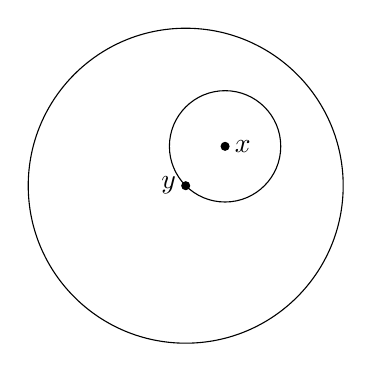
\begin{tikzpicture}
        \filldraw (0.5, 0.5) circle (0.05) node[right] {\( x \)};
        \draw (0.5, 0.5) circle (0.707);

        \filldraw (0, 0) circle (0.05) node[left] {\( y \)};
        \draw (0, 0) circle (2);
      \end{tikzpicture}
      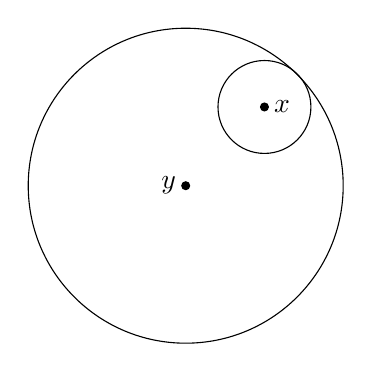
\begin{tikzpicture}
        \filldraw (1, 1) circle (0.05) node[right] {\( x \)};
        \draw (1, 1) circle (0.59);

        \filldraw (0, 0) circle (0.05) node[left] {\( y \)};
        \draw (0, 0) circle (2);
      \end{tikzpicture}
    \end{Center}
  \end{description}
\end{proof}

\begin{proposition}\label{thm:locally_countable_metric_topology}
  The following is an alternative base for the metric topology\Tinyref{def:metric_topology}:

  \begin{equation*}
    \Cal{B}(x) \coloneqq \{ B (x, \tfrac 1 n) \colon n = 1, 2, 3, \ldots \}.
  \end{equation*}
\end{proposition}
\begin{proof}
  The proof is the same as in \cref{def:metric_topology}, except for a slight tweak in \ref{thm:topological_local_base_axioms/BP3}, where we define \( m \) to be the the smallest positive integer such that
  \begin{equation*}
    \tfrac 1 m \leq \min\{ \mu(x, y), r - \mu(x, y) \}.
  \end{equation*}

  Note that \( m \) exists by \cref{thm:ordinals_are_well_ordered}.

  We then obtain \( B(x, \tfrac 1 m) \subseteq B(y, \tfrac 1 n) \).
\end{proof}

\begin{proposition}\label{thm:metric_topology_properties}
  The metric topology \( \Cal{T} \) on \( X \) induced by \( \mu \) has the following properties:
  \begin{defenum}
    \DItem{thm:metric_topology_properties/ball_is_open} For every point \( x \in X \) and any radius \( r > 0 \), the ball \( B(x, r) \) is an open set and, hence, a neighborhood of \( x \).
    \DItem{thm:metric_topology_properties/first_countable} \( \Cal{T} \) is first-countable.
    \DItem{thm:metric_topology_properties/hausdorff} \( \Cal{T} \) is Hausdorff.
  \end{defenum}
\end{proposition}
\begin{proof}
  \begin{description}
    \RItem{thm:metric_topology_properties/ball_is_open} Obvious from \cref{def:metric_topology}.

    \RItem{thm:metric_topology_properties/first_countable} Since \cref{thm:locally_countable_metric_topology} involves generating a topology using a neighborhood system of countable local neighborhoods, \( \Cal{T} \) is first-countable.

    \RItem{thm:metric_topology_properties/hausdorff} Let \( x, y \in X \) be distinct points. Define
    \begin{equation*}
      r \coloneqq \dfrac 1 2 \mu(x, y),
    \end{equation*}
    so that
    \begin{equation*}
      B(x, r) \cap B(y, r) = \varnothing.
    \end{equation*}
  \end{description}
\end{proof}

\begin{proposition}\label{thm:metric_convergence_iff_metric_topology_convergence}
  Let \( (X, \mu) \) be a metric space and \( \Cal{T} \) be the induced metric topology\Tinyref{def:metric_topology}. The convergence\Tinyref{subsec:convergence} in \( \Cal{T} \) is the completely described by sequences, that is,

  \begin{defenum}
    \DItem{thm:metric_convergence_iff_metric_topology_convergence/single_limit} every converging net\Tinyref{def:topological_net} has a single limit.

    \DItem{thm:metric_convergence_iff_metric_topology_convergence/cluster_point} \( x \in X \) is a cluster point\Tinyref{def:net_cluster_point} of the sequence \( \{ x_i \}_{i=1}^\infty \) if and only if for every positive real number \( \varepsilon > 0 \) and every index \( i_0 \) there exists an index \( i_\varepsilon > i_0 \) such that
    \begin{equation*}
      \mu(x, x_{i_\varepsilon}) < \varepsilon.
    \end{equation*}

    \DItem{thm:metric_convergence_iff_metric_topology_convergence/limit_point} \( x \in X \) is a limit point\Tinyref{def:net_limit_point} of the sequence \( \{ x_i \}_{i=1}^\infty \) if and only if for every positive real number \( \varepsilon > 0 \) there exists an index \( i_0 \) such that
    \begin{equation*}
      i \geq i_0 \implies \mu(x, x_i) < \varepsilon.
    \end{equation*}

    \DItem{thm:metric_convergence_iff_metric_topology_convergence/closure} given any set \( A \subseteq X \), a point \( x \in X \) belongs to \( \Cl{A} \) if and only if there exists a sequence \( \{ x_i \}_{i=1}^\infty \subseteq A \) such that \( x_i \xrightarrow[i \to \infty]{} x \) (compare with \cref{thm:limit_point_iff_in_closure}).
  \end{defenum}
\end{proposition}
\begin{proof}
  \begin{description}
    \RItem{thm:metric_convergence_iff_metric_topology_convergence/single_limit} Follows directly from \cref{thm:t2_iff_singleton_limits} and \cref{thm:metric_topology_properties/hausdorff}.

    \RItem{thm:metric_convergence_iff_metric_topology_convergence/cluster_point} Fix a sequence \( x_i \to x \).

    \begin{description}
      \Implies Fix a radius \( \varepsilon > 0 \) and an index \( i_0 \). Note that \( B(x, \varepsilon) \) is a neighborhood of \( x \) and hence by \cref{def:net_cluster_point} there exists an index \( i_\varepsilon \geq i_0 \) such that \( x_{i_U} \in B(x, \varepsilon) \), which is the same as
      \begin{equation*}
        \mu(x, x_{i_U}) < \varepsilon.
      \end{equation*}

      \ImpliedBy Fix a neighborhood \( U \) of \( x \). Since the topology is generated by a local base of balls, then \( U \) contains some ball \( B(x, r) \). Thus there exists an index \( i_0 \), such that
      \begin{equation*}
        \mu(x, x_{i_r}) < r,
      \end{equation*}
      hence
      \begin{equation*}
        x_{i_r} \in B(x, r) \subseteq U.
      \end{equation*}
    \end{description}

    \RItem{thm:metric_convergence_iff_metric_topology_convergence/limit_point} Similar to \ref{thm:metric_convergence_iff_metric_topology_convergence/cluster_point}.

    \RItem{thm:metric_convergence_iff_metric_topology_convergence/closure}
    \begin{description}
      \Implies Fix a nonempty set \( A \) and \( x \in \Cl A \). If \( x \in A \), then the constant sequence with all members equal to \( x \) converges to \( A \).

      Assume that \( x \not\in A \) and choose any sequence\AOC
      \begin{equation*}
        x_i \in B(x, \tfrac 1 i) \setminus \{ x \}, i = 1, 2, \ldots.
      \end{equation*}

      Fix \( \varepsilon > 0 \). By \cref{thm:ordinals_are_well_ordered} there exists a least positive integer \( i_0 \) such that \( \tfrac 1 i_0 < \varepsilon \). It follows that \( x_i \to x \) since
      \begin{equation*}
        i \geq i_0 \implies \mu(x, x_i) \leq \mu(x, x_{i_0}) \leq \varepsilon.
      \end{equation*}

      \ImpliedBy Obvious
    \end{description}
  \end{description}
\end{proof}

\begin{definition}\label{def:isometry}\cite[253]{Engelking1989}
  Let \( (X, \mu) \) and \( (Y, \nu) \) be two metric spaces\Tinyref{def:metric_space}. We say that the function \( f: X \to Y \) is a \textbf{distance preserving map} or \textbf{isometry} or \textbf{isometric embedding} if
  \begin{equation*}
    \forall x, y \in X, \mu(x, y) = \nu(f(x), f(y)).
  \end{equation*}

  If \( f \) is bijective, we say that \( X \) and \( Y \) are \textbf{isometric}.
\end{definition}

\begin{proposition}\label{def:isometry_is_injective}
  An isometry\Tinyref{def:isometry} \( f: (X, \mu) \to (Y, \nu) \) is always injective.
\end{proposition}
\begin{proof}
  If\LEM \( f(x) = f(x') \), then by \ref{def:metric_space/identity}, \( x = x' \).
\end{proof}

\begin{definition}\label{def:category_of_metric_spaces}
  The class\Tinyref{def:set_zfc} of all metric spaces forms the category\Tinyref{def:category} \( \Bold{Met} \), where for every two metric spaces \( X, Y \in \Bold{Met} \), the morphisms \( \Bold{Met}(X, Y) \) are the isometries\Tinyref{def:isometry} from \( X \) to \( Y \) and composition is the usual function composition\Tinyref{def:function_composition}.

  The category is concrete\Tinyref{def:concrete_category} and locally small\Tinyref{def:category_cardinality}.
\end{definition}

\begin{definition}\label{def:equivalent_metrics}
  Two metrics \( \mu \) and \( \nu \) on the set \( X \) are said to be \textbf{equivalent} if \( \mu \) and \( \nu \) have the same metric topology\Tinyref{def:metric_topology}. They are said to be \textbf{strongly equivalent} if there exist constants \( \alpha, \beta \in \BB{R} \) such that for every \( x, y \in X \) we have
  \begin{equation*}
    \alpha \nu(x, y) \leq \mu(x, y) \leq \beta \nu(x, y).
  \end{equation*}
\end{definition}

\begin{theorem}\label{thm:real_metric_and_order_topologies_coincide}
  For the real numbers, the metric\Tinyref{def:metric_topology} and order\Tinyref{def:order_topology} topologies coincide.
\end{theorem}
\begin{proof}
  The metric topology \( \Cal{T}_M \) is generated by the base\Tinyref{def:topological_base}
  \begin{equation*}
    \Cal{B} \coloneqq \{ B(x, r) \colon x \in \BB{R}, r \in \BB{R}^{>0} \}
  \end{equation*}
  and the order topology \( \Cal{T}_O \) is generated by the subbase\Tinyref{def:topological_subbase}
  \begin{equation*}
    \Cal{P} \coloneqq \{ (a, \infty) \colon a \in \BB{R} \} \cup \{ (\infty, b) \colon b \in \BB{R} \}.
  \end{equation*}

  The inclusion \( \Cal{B} \subseteq FI(\Cal{P}) \) is obvious since any ball \( B(x, r) \) is the intersection of the two rays
  \begin{equation*}
    B(x, r) = (x - r, \infty) \cap (-\infty, x + r).
  \end{equation*}

  Thus \( \Cal{T}_M \subseteq \Cal{T}_O \). We now only need to show that \( \Cal{B} \) is a base for \( \Cal{T}_O \).

  Let \( U \in \Cal{T}_O \). Since \( FI(\Cal{P}) \) is a base for \( \Cal{T}_O \), there exists\Tinyref{def:topological_base/union} a family \( \{ U_i \}_{i \in I} \subseteq FI(\Cal{P}) \) such that
  \begin{equation*}
    U = \bigcup_{i \in I} U_i.
  \end{equation*}

  We only need to express every \( U_i \) as a union of balls from \( \Cal{B} \). There are several possibilities:
  \begin{itemize}
    \item if \( U_i \) is the open interval \( (a, \infty) \),
    \begin{equation*}
      (a, \infty) = \bigcup_{i=1}^\infty B(a + i, 1).
    \end{equation*}

    \item if \( U_i \) is the open interval \( (-\infty, b) \),
    \begin{equation*}
      (-\infty, b) = \bigcup_{i=1}^\infty B(b - i, 1).
    \end{equation*}

    \item if \( U_i \) is the intersection \( (a, \infty) \cap (-\infty, b), a < b \),
    \begin{equation*}
      (a, \infty) \cap (-\infty, b) = B(\tfrac {a + b} 2, \tfrac {b - a} 2)
    \end{equation*}

    \item if \( U_i \) is the empty set,
    \begin{equation*}
      \varnothing = \bigcup \varnothing \text{ (see \cref{def:set_union})}.
    \end{equation*}
  \end{itemize}

  Thus \( U_i \) is the union of an at most countable amount of balls. The countable union of countable sets is again countable, hence by \cref{def:topological_base/union}, \( \Cal{B} \) is a base for \( \Cal{T}_O \).
\end{proof}

\begin{definition}\label{def:fundamental_sequence}
  Let \( (X, \mu) \) be a metric space. We say that the sequence \( \{ x_i \}_{i=1}^n \subseteq X \) is a \textbf{fundamental sequence} or \textbf{Cauchy sequence} if, for any \( \varepsilon > 0 \), there exists an index \( i_0 \) such that
  \begin{equation*}
    i, j \geq i_0 \implies \mu(x_i, x_j) < \varepsilon.
  \end{equation*}
\end{definition}

\begin{proposition}\label{thm:fundamental_sequence_is_bounded}
  Any fundamental sequence \( \{ x_i \}_{i=1}^n \) is bounded\Tinyref{def:metric_space/bounded_sequence}.
\end{proposition}
\begin{proof}
  Fix \( \varepsilon > 0 \). There exists an index \( i_0 \) such that
  \begin{equation*}
    i, j \geq i_0 \implies \mu(x_i, x_j) < \varepsilon.
  \end{equation*}

  Since the set
  \begin{equation*}
    I \coloneqq \{ x_i \colon i \leq i_0 \}
  \end{equation*}
  is finite, it has a finite diameter\Tinyref{def:metric_space/diameter}.

  Let \( i < i_0 \) and \( j \geq i_0 \). Then
  \begin{equation*}
    \mu(x_i, x_j) \leq \mu(x_i, x_{i_0}) + \mu(x_{i_0}, x_j) < \Diam(I) + \varepsilon,
  \end{equation*}
  which is a finite number.

  Thus the distance between any two elements of the sequence is finite and the sequence is bounded.
\end{proof}

\begin{proposition}\label{thm:fundamental_subsequence_convergence}
  In any metric space\Tinyref{def:complete_metric_space}, a fundamental sequence\Tinyref{def:fundamental_sequence} converges to a value if and only if it has a subsequence that converges to the same value.
\end{proposition}
\begin{proof}
  Let \( (X, \mu) \) be a metric space and let \( \{ x_i \}_{i=1}^\infty \) be a fundamental sequence.

  \begin{description}
    \Implies Obvious
    \ImpliedBy Assume that the subsequence \( \{ x_{i_k} \}_{k=1}^\infty \) converges to \( x \). Fix \( \varepsilon > 0 \). There exist \( i_0 \) and \( k_0 \) such that
    \begin{align*}
      &i, j \geq i_0 \implies \mu(x_i, x_j) < \tfrac \varepsilon 2 \\
      &k \geq k_0 \implies \mu(x, x_{i_k}) < \tfrac \varepsilon 2
    \end{align*}

    Fix \( i \geq i_0 \) and let \( k \geq k_0 \) be such that \( i_k \geq i_0 \). Then
    \begin{equation*}
      \mu(x, x_i) \leq \mu(x, x_{i_k}) + \mu(x_{i_k}, x_i) < \varepsilon.
    \end{equation*}

    Since \( \varepsilon \) was arbitrary, we conclude that \( \lim_{i \to \infty} x_i = \lim_{k \to \infty} x_{i_k} = x \).
  \end{description}
\end{proof}

\begin{definition}\label{def:complete_metric_space}
  We say that a metric space is \textbf{complete} if every fundamental sequence\Tinyref{def:fundamental_sequence} has a limit\Tinyref{thm:metric_convergence_iff_metric_topology_convergence/limit_point}.

  An isometry \( f: X \to Y \) is called a \textbf{completion of \( X \)} if \( Y \) is complete and \( f(X) \) is dense\Tinyref{def:topologically_dense_set/dense} in \( Y \) (see \cref{thm:metric_space_completion_existence}).
\end{definition}

\begin{proposition}\label{thm:convergent_sequence_is_fundamental}
  In a complete metric space\Tinyref{def:complete_metric_space}, every convergent\Tinyref{def:net_limit_point}\Tinyref{thm:metric_convergence_iff_metric_topology_convergence/limit_point} sequence is fundamental\Tinyref{def:fundamental_sequence}.
\end{proposition}
\begin{proof}
  Let \( (X, \mu) \) be a complete metric space and \( \{ x_i \}_{i=1}^\infty \) be a sequence that converges to \( x \). Fix \( \varepsilon > 0 \). Then there exists an index \( i_0 \) such that
  \begin{equation*}
    i \geq i_0 \implies \mu(x, x_i) < \tfrac \varepsilon 2.
  \end{equation*}

  Then
  \begin{equation*}
    i, j \geq i_0 \implies \mu(x_i, x_j) \leq \mu(x_i, x) + \mu(x, x_j) < \tfrac \varepsilon 2 + \tfrac \varepsilon 2 = \varepsilon.
  \end{equation*}

  Since \( \varepsilon > 0 \) was arbitrary, we conclude that the sequence is fundamental.
\end{proof}

\begin{corollary}[Cauchy convergence criterion]\label{thm:cauchy_convergence_criterion}
  A sequence in a complete metric space is convergent\Tinyref{def:net_limit_point}\Tinyref{thm:metric_convergence_iff_metric_topology_convergence/limit_point} if and only if it is a fundamental sequence\Tinyref{def:fundamental_sequence}.
\end{corollary}
\begin{proof}
  \Implies Given by \cref{thm:convergent_sequence_is_fundamental}
  \ImpliedBy Given by \cref{def:complete_metric_space}
\end{proof}

\begin{theorem}[Cantor]\label{thm:cantor_nested_compacts}
  A descending sequence of nonempty compact sets \( F_1 \supseteq F_2 \supseteq \ldots \) in a complete metric space such that \( \Diam(F_i) \to 0 \) intersects at exactly one point (compare with \cref{thm:noncompact_kuratowski_lemma}).
\end{theorem}
\begin{proof}
  Choose\AOC an element \( x_i \in F_i \) for any \( i = 1, 2, \ldots \). Then the sequence \( \{ x_i \}_{i=1}^\infty \) is fundamental. To see this, let \( \varepsilon > 0 \) and let \( i_0 \) be an index such that \( \Diam(F_{i_0}) < \varepsilon \). Then if \( j \geq i \geq i_0 \), \( x_j \) is contained in \( F_i \) and \( \mu(x_i, x_j) < \varepsilon \). Thus the sequence is indeed fundamental and, since the space is complete, it has a limit point \( x \).

  The point \( x \) is contained in every set \( F_i, i = 1, 2, \ldots \) since all of the sets \( F_i \) are closed (by \cref{thm:complete_metric_space_compact_conditions}) and contain their limit points\Tinyref{thm:limit_point_iff_in_closure}. Thus
  \begin{equation*}
    x \in \bigcap_{i=1}^\infty F_i.
  \end{equation*}

  Furthermore,
  \begin{equation*}
    \Diam\left( \bigcap_{i=1}^\infty F_i \right) = 0,
  \end{equation*}
  hence \( x \) is the only point in the intersection.
\end{proof}

\begin{theorem}\label{thm:metric_space_completion_existence}
  Every metric space has a completion\Tinyref{def:complete_metric_space}.
\end{theorem}
\begin{proof}
  Let \( (X, \mu) \) be a metric space.

  \begin{defenum}
    \DItem{thm:metric_space_completion_existence/part_a} First, we build the pseudometric space \( (F, \rho) \). We deal with fundamental sequences and isometries in pseudometric spaces, where the definitions, however, does not change.

     Define \( F \) to be the set of all fundamental sequences\Tinyref{def:fundamental_sequence} in X. Define the pseudometric
    \begin{align*}
      &\rho: F \times F \to \BB{R}^{\geq 0} \\
      &\rho\left( \{ x_i \}_{i=1}^\infty, \{ y_i \}_{i=1}^\infty \right) \coloneqq \lim_{i \to \infty} \mu(x_i, y_i).
    \end{align*}

    We first show that is well defined as a function\Tinyref{def:function}. Let \( \{ x_i \}_{i=1}^\infty \) and \( \{ y_i \}_{i=1}^\infty \) be two sequences. Fix \( \varepsilon > 0 \). Then there exists an \( i_0 \) such that
    \begin{equation*}
      i, j \geq i_0 \implies \mu(x_i, x_i) < \tfrac \varepsilon 2 \text{ and } \mu(y_i, y_j) < \tfrac \varepsilon 2.
    \end{equation*}

    Fix \( i, j \geq i_0 \). Then
    \begin{equation*}
      \mu(x_i, y_i) \leq \mu(x_i, x_j) + \mu(x_j, y_j) + \mu(y_j, y_i) < \mu(x_j, y_j) + \varepsilon,
    \end{equation*}
    hence
    \begin{equation*}
      \Abs{\mu(x_i, y_i) - \mu(x_j, y_j)} < \varepsilon.
    \end{equation*}

    Thus the sequence \( \{ \mu(x_i, y_i) \}_{i=1}^\infty \) is fundamental and, by \cref{def:real_numbers_complete_metric_space}, it is convergent.

    Now we check that \( \rho \) is indeed a pseudometric:
    \begin{description}
      \RItem{def:metric_space/pseudometric_identity} For every sequence \( x \in F \),
      \begin{equation*}
        \rho(x, x) = \lim_{i \to \infty} \mu(x_i, x_i) = 0.
      \end{equation*}
      \RItem{def:metric_space/symmetry} For all sequences \( x, y \in F \),
      \begin{equation*}
        \rho(x, y) = \lim_{i \to \infty} \mu(x_i, y_i) = \lim_{i \to \infty} \mu(y_i, x_i) = \rho(y, x).
      \end{equation*}

      \RItem{def:metric_space/triangle_inequality} For all sequences \( x, y, z \in F \),
      \begin{equation*}
        \rho(x, z) = \lim_{i \to \infty} \mu(x_i, z_i) \leq \lim_{i \to \infty} \mu(x_i, y_i) + \lim_{i \to \infty} \mu(y_i, z_i) = \rho(x, y) + \rho(y, z).
      \end{equation*}
    \end{description}

    \DItem{thm:metric_space_completion_existence/part_b} We prove that every fundamental sequence in \( (F, \rho) \) is convergent.

    Let \( \{ c^{(i)} \}_{i=1}^\infty \) be a fundamental sequence (of sequences) in \( (F, \rho) \). Thus, for every \( i = 1, 2, \ldots \), there exists an index \( n_i \) such that
    \begin{equation*}
      j \geq n_i \implies \mu(c_j^{(i)}, c_{n_i}^{(i)}) < \tfrac 1 i.
    \end{equation*}

    Define the sequence
    \begin{equation*}
      d_i \coloneqq c_{n_i}^{(i)}, i = 1, 2, \ldots.
    \end{equation*}

    To see that it is fundamental, fix \( \varepsilon > 0 \). Now since the sequence \( \{ c^{(i)} \} \) in \( F \) is fundamental, there exists \( i_0 \) such that
    \begin{equation*}
      i, j \geq i_0 \implies \rho(c^{(i)}, c^{(j)}) = \lim_{k \to \infty} \mu(c_k^{(i)}, c_k^{(j)}) < \frac \varepsilon 2.
    \end{equation*}

    Let \( j_0 \geq i_0 \) be an index such that
    \begin{equation*}
      \frac 2 {j_0} < \frac \varepsilon 2.
    \end{equation*}

    Fix \( i \geq j \geq j_0 \). Let \( l \geq \max \{ n_i, n_j \} \) be such that
    \begin{equation*}
      \mu(c_l^{(i)}, c_l^{(j)}) < \frac \varepsilon 2.
    \end{equation*}

    Then
    \begin{align*}
      \mu(d_i, d_j)
      &=
      \mu(c_{n_i}^{(i)}, c_{n_j}^{(j)})
      \leq \\ &\leq
      \mu(c_{n_i}^{(i)}, c_l^{(i)}) + \mu(c_l^{(i)}, c_l^{(j)}) + \mu(c_l^{(j)}, c_{n_j}^{(j)})
      \leq \\ &\leq
      \frac 1 i + \frac \varepsilon 2 + \frac 1 j
      \leq
      \frac 2 j + \frac \varepsilon 2
      <
      \varepsilon.
    \end{align*}

    Thus we have
    \begin{equation*}
      i \geq j \geq j_0 \implies \mu(d_i, d_j) < \varepsilon,
    \end{equation*}
    which proves that the sequence \( \{ d_i \}_{i=1}^\infty \) is fundamental in \( (X, \mu) \).

    Now it remains to show that \( c^{(i)} \xrightarrow[i \to \infty]{} d \) in \( (F, \rho) \).

    Fix \( \varepsilon > 0 \) and let \( i_0 \) be such that
    \begin{equation*}
      \frac 1 {i_0} \leq \frac \varepsilon 2.
    \end{equation*}
    and
    \begin{equation*}
      i, j \geq i_0 \implies \mu(d_i, d_j) < \frac \varepsilon 2.
    \end{equation*}

    Now fix \( i \geq i_0 \). We have, for all \( k \geq i \),
    \begin{align*}
      \mu(c_{n_k}^{(i)}, d_k)
      &=
      \mu(c_{n_k}^{(i)}, c_{n_k}^{(k)})
      \leq \\ &\leq
      \mu(c_{n_k}^{(i)}, c_{n_i}^{(i)}) + \mu(c_{n_i}^{(i)}, c_{n_k}^{(k)})
      = \\ &=
      \mu(c_{n_k}^{(i)}, c_{n_i}^{(i)}) + \mu(d_i, d_k)
      < \\ &<
      \frac 1 i + \frac \varepsilon 2
      <
      \varepsilon.
    \end{align*}

    Hence
    \begin{align*}
      \rho(c^{(i)}, d)
      =
      \lim_{k \to \infty} \mu(c_k^{(i)}, d_k)
      =
      \lim_{k \to \infty} \mu(c_k^{(i)}, c_{n_k}^{(k)})
      <
      \varepsilon.
    \end{align*}

    Thus, given \( \varepsilon > 0 \), we found an index \( i_0 \) such that
    \begin{equation*}
      i \geq i_0 \implies \rho(c^{(i)}, d) < \varepsilon.
    \end{equation*}

    Thus \( d = \lim_{i \to \infty} c^{(i)} \) and \( (F, \rho) \) is a complete pseudometric space.

    \DItem{thm:metric_space_completion_existence/part_c} We construct an isometry of \( (X, \mu) \) into \( (F, \rho) \).

    Define the function
    \begin{align*}
      &\iota: X \to F \\
      &\iota(x) \coloneqq (x, x, x, \ldots),
    \end{align*}
    which sends each element of \( X \) into the corresponding constant sequence in \( F \).

    It is an isometry\Tinyref{def:isometry} since
    \begin{equation*}
      \rho(\iota(x),\iota(y)) = \lim_{i \to \infty} \mu(x, y) = \mu(x, y).
    \end{equation*}

    \DItem{thm:metric_space_completion_existence/part_d} We show that the image \( \iota(X) \) is dense in \( (F, \rho) \).

    Fix the fundamental sequence \( y \coloneqq \{ y_i \}_{i=1}^\infty \). Define the sequence \( x \) of sequences
    \begin{equation*}
      x^{(i)} \coloneqq \iota(y_i), i = 1, 2, \ldots.
    \end{equation*}

    It is fundamental in \( (F, \rho) \) since \( e \) is an isometry and since \( y \) is fundamental in \( (X, \mu) \).

    Fix \( \varepsilon > 0 \). Let \( i_0 \) be such that
    \begin{equation*}
      i, j \geq i_0 \implies \mu(y_i, y_j) < \varepsilon.
    \end{equation*}

    For \( i, k \geq i_0 \), we have
    \begin{align*}
      \mu(x_k^{(i)}, y_k)
      \leq
      \mu(x_k^{(i)}, y_i) + \mu(y_i, y_k)
      =
      0 + \mu(y_i, y_k)
      <
      \varepsilon,
    \end{align*}
    hence
    \begin{equation*}
      \rho(x^{(i)}, y) = \lim_{k \to \infty} \mu(x_k^{(i)}, y_k) < \varepsilon.
    \end{equation*}

    We conclude that \( x^{(i)} \xrightarrow[i \to \infty]{} y \) in \( (F, \rho) \), which implies that \( e(X) \) is dense in \( (F, \rho) \).

    \DItem{thm:metric_space_completion_existence/part_e} We build a complete metric space \( (C, \nu) \) from \( (F, \rho) \).

    We use \cref{thm:pseudometric_to_metric} to construct a complete metric space \( (C, \nu) \) from the complete pseudometric space \( (F, \rho) \).

    We adapt \( \iota \) to the equivalence classes on \( C \):
    \begin{align*}
      &\hat\iota: X \to C \\
      &\hat\iota(x) \coloneqq [\iota(x)].
    \end{align*}

    Thus \( \hat\iota \) embeds \( X \) into the complete metric space \( C \).
  \end{defenum}
\end{proof}

\begin{proposition}\label{thm:metric_space_completion_uniqueness}
  Let \( X \) be a metric space. If both \( f: X \to Y \) and \( g: X \to Z \) are completions\Tinyref{def:complete_metric_space} of \( X \), then \( Y \) and \( Z \) are isometric.
\end{proposition}
\begin{proof}
  Let \( y \in Y \) and let \( \{ x_i \}_{i \to \infty} \subseteq X \) be a sequence such that
  \begin{equation*}
    f(x_i) \xrightarrow[i \to \infty]{} y.
  \end{equation*}

  Such a sequence exists since \( f(X) \) is dense in \( Y \).

  Define \( z \coloneqq \lim_{i \to \infty} g(x_i) \). Since both \( f \) and \( g \) are isometries, \( z \) does not depend on the choice of sequence \( \{ x_i \}_{i \to \infty} \) such that \( f(x_i) \to y \). Furthermore, if \( z \in Z \) is given rather than \( y \in Y \), an analogous process allows us to determine \( y \) uniquely based on \( z \).

  Thus we have a bijective isometry between \( Y \) and \( Z \).
\end{proof}
